\documentclass{article}

% Language setting
% Replace `english' with e.g. `spanish' to change the document language
\usepackage[english]{babel}

% Set page size and margins
% Replace `letterpaper' with `a4paper' for UK/EU standard size
\usepackage[letterpaper,top=2cm,bottom=2cm,left=3cm,right=3cm,marginparwidth=1.75cm]{geometry}

% Useful packages
\usepackage{amsmath}
\usepackage{graphicx}
\usepackage[colorlinks=true, allcolors=blue]{hyperref}
\usepackage{xcolor}
\usepackage{datetime}
\usepackage[section]{placeins} 
\usepackage{pdfpages}
\usepackage{float}

\title{ME136 Lab 5}
\author{Nathan Yacovetta, Aarchan Saxena, Jobanpreet Mutti, Radhika Marolia}
\date{December 1, 2023}

\begin{document}
\maketitle

\section{Contributions}

\begin{itemize}
\item Nathan Yacovetta: Performed lab tasks, optimized hover time, and completed deliverables.
\item Aarchan Saxena: Performed lab tasks, optimized hover time, and completed deliverables.
\item Jobanpreet Mutti: Performed lab tasks, optimized hover time, and completed deliverables.
\item Radhika Marolia: Worked on lab tasks and helped write up report.
\end{itemize}

\section{Experimental Set-up:}
\subsection{Description}
For our experimental set-up, we centered the drone in the middle of the flight space and turned the vehicle on. Once on, we allowed the drone to fly for as long as possible.


\subsection{Screenshost}
\begin{figure} [H]
\centering
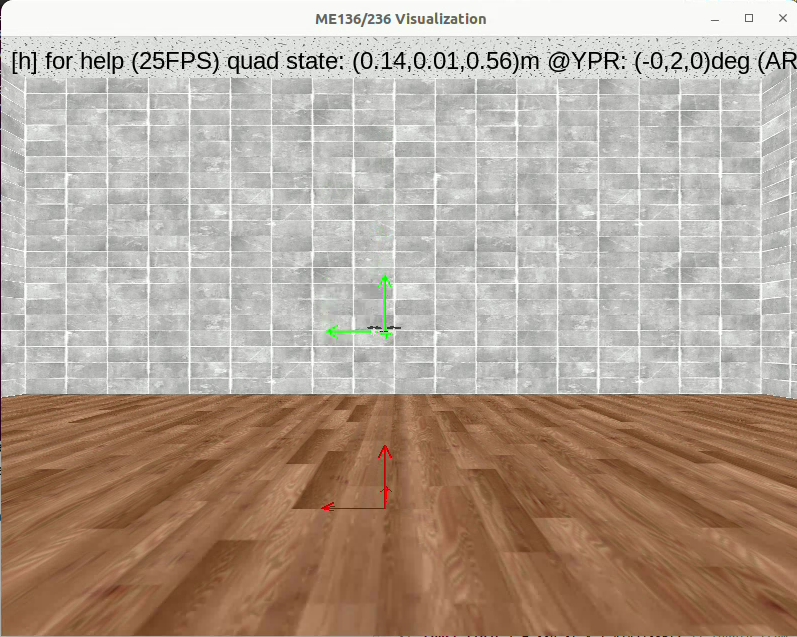
\includegraphics[scale=.60]{ME136Lab5HoverScreenshot.png}
\caption{Experimental Set-Up with Vehicle On}
\end{figure}
\FloatBarrier
\vspace{24pt}

\section{Height Estimator}

\subsection{Part A}
To collect the data for the plots in 3.2, we began the simulator, picked up the vehicle approximately 0.5 m above the surface, held it there for 5 seconds, rotated it through a pitch and roll angle of $\pm$ 30 degrees, and smoothly returned it to the ground. 

\subsection{Part B}

\begin{itemize}
\item The roll and pitch estimates
\begin{figure} [H]
\centering
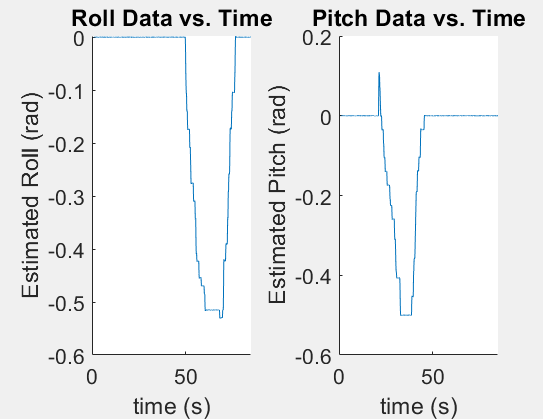
\includegraphics[scale=.75]{ME136_Lab5_Q3bi.png}
\caption{Estimated Roll and Pitch VS Time}
\end{figure}
\FloatBarrier
\vspace{24pt}

\item The vertical velocity
\begin{figure} [H]
\centering
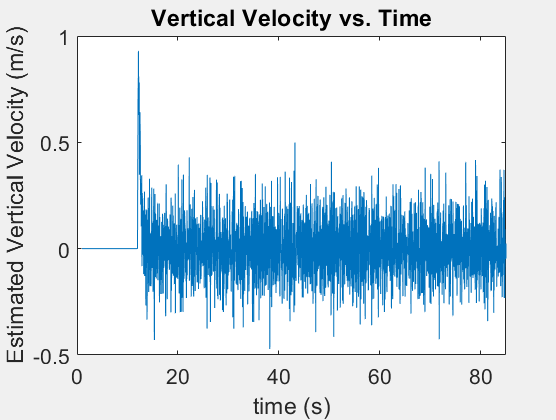
\includegraphics[scale=.75]{ME136_Lab5_Q3bii.png}
\caption{Estimated Vertical Velocity VS Time}
\end{figure}
\FloatBarrier
\vspace{24pt}

\item The height estimate and the measurements from the distance sensor
\begin{figure} [H]
\centering
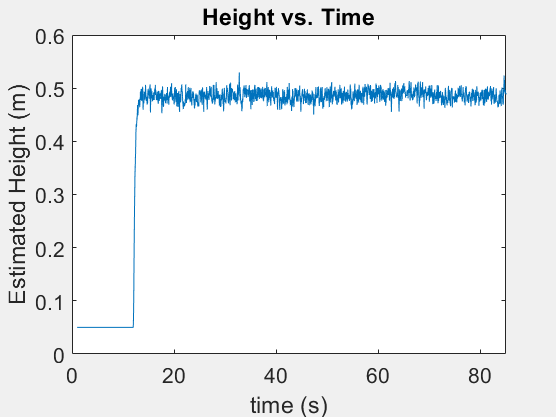
\includegraphics[scale=.75]{ME136_Lab5_Q3biii.png}
\caption{Estimated Height VS Time}
\end{figure}
\FloatBarrier
\vspace{24pt}

\end{itemize}



\subsection{Part C}
During the time period of our experiment, the estimator measurements appear to be accurate and there are no significant disruptions.

\section{Horizontal Estimator}
\subsection{Part A}
To collect the data for the plots in 4.2, we began the simulator, picked up the vehicle approximately 0.5 m above the surface, and held it there for 2 seconds. Keeping the vehicle orientation constant, we walked forward about 1m, stopped for 2 seconds, walked left about 1 m, stopped for 2 seconds, rotated it through a pitch and roll angle of $\pm$ 30 degrees, and smoothly returned it to the ground. 


\subsection{Part B}
\begin{itemize}
\item The rate gyroscope measurements
\begin{figure} [H]
\centering
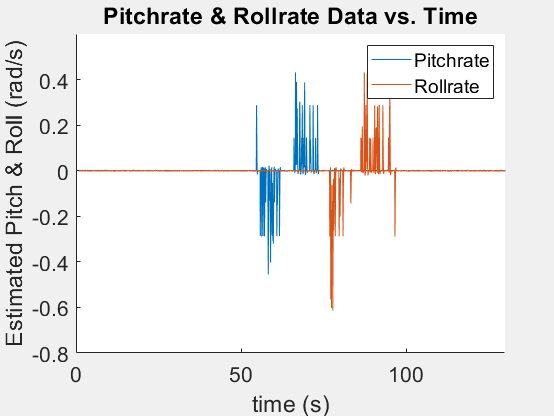
\includegraphics[scale=.75]{ME136_Lab5_Q4bi.png}
\caption{Estimated Pitchrate and Rollrate VS Time}
\end{figure}
\FloatBarrier
\vspace{24pt}

\item The output from the flow sensor
\begin{figure} [H]
\centering
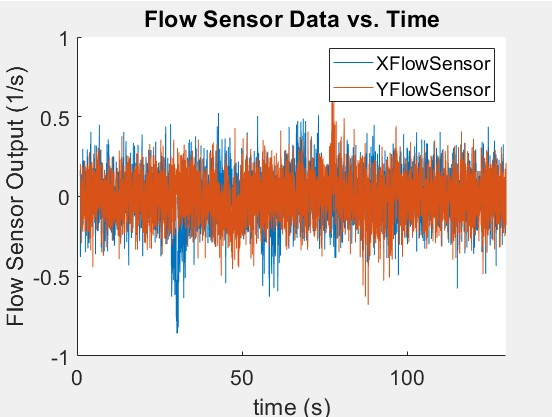
\includegraphics[scale=.75]{ME136_Lab5_Q4bii.jpg}
\caption{Flow Sensor Data VS Time}
\end{figure}
\FloatBarrier
\vspace{24pt}

\item The estimated horizontal velocity
\begin{figure} [H]
\centering
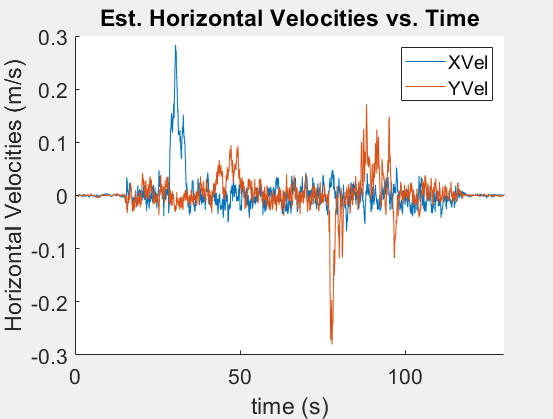
\includegraphics[scale=.75]{ME136_Lab5_Q4biii.png}
\caption{Estimated Horizontal Velocities VS Time}
\end{figure}
\FloatBarrier
\vspace{24pt}

\item The height estimate
\begin{figure} [H]
\centering
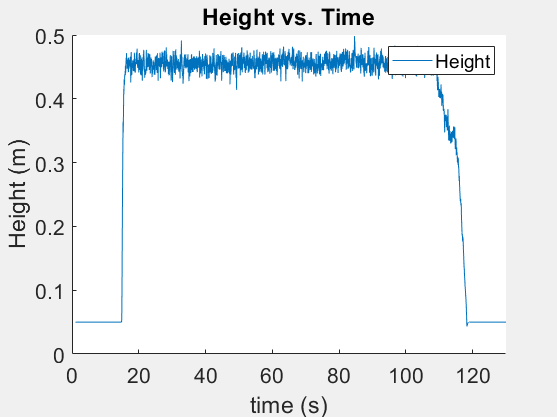
\includegraphics[scale=.75]{ME136_Lab5_Q4biv.png}
\caption{Height Estimate VS Time}
\end{figure}
\FloatBarrier
\vspace{24pt}

\end{itemize}


\subsection{Part C}
During the time period of our experiment, the estimator measurements appear to be accurate and there are no significant disruptions.



\section{Closed-loop Hover Flight}

\subsection{Part A}
To collect the data for the plots in 5.2, we placed the vehicle on the floor in the center of the flight space, turned it on, and let it fly for as long as possible.

\subsection{Part B}
\begin{itemize}
\item The estimated angles and desired angles
\begin{figure} [H]
\centering
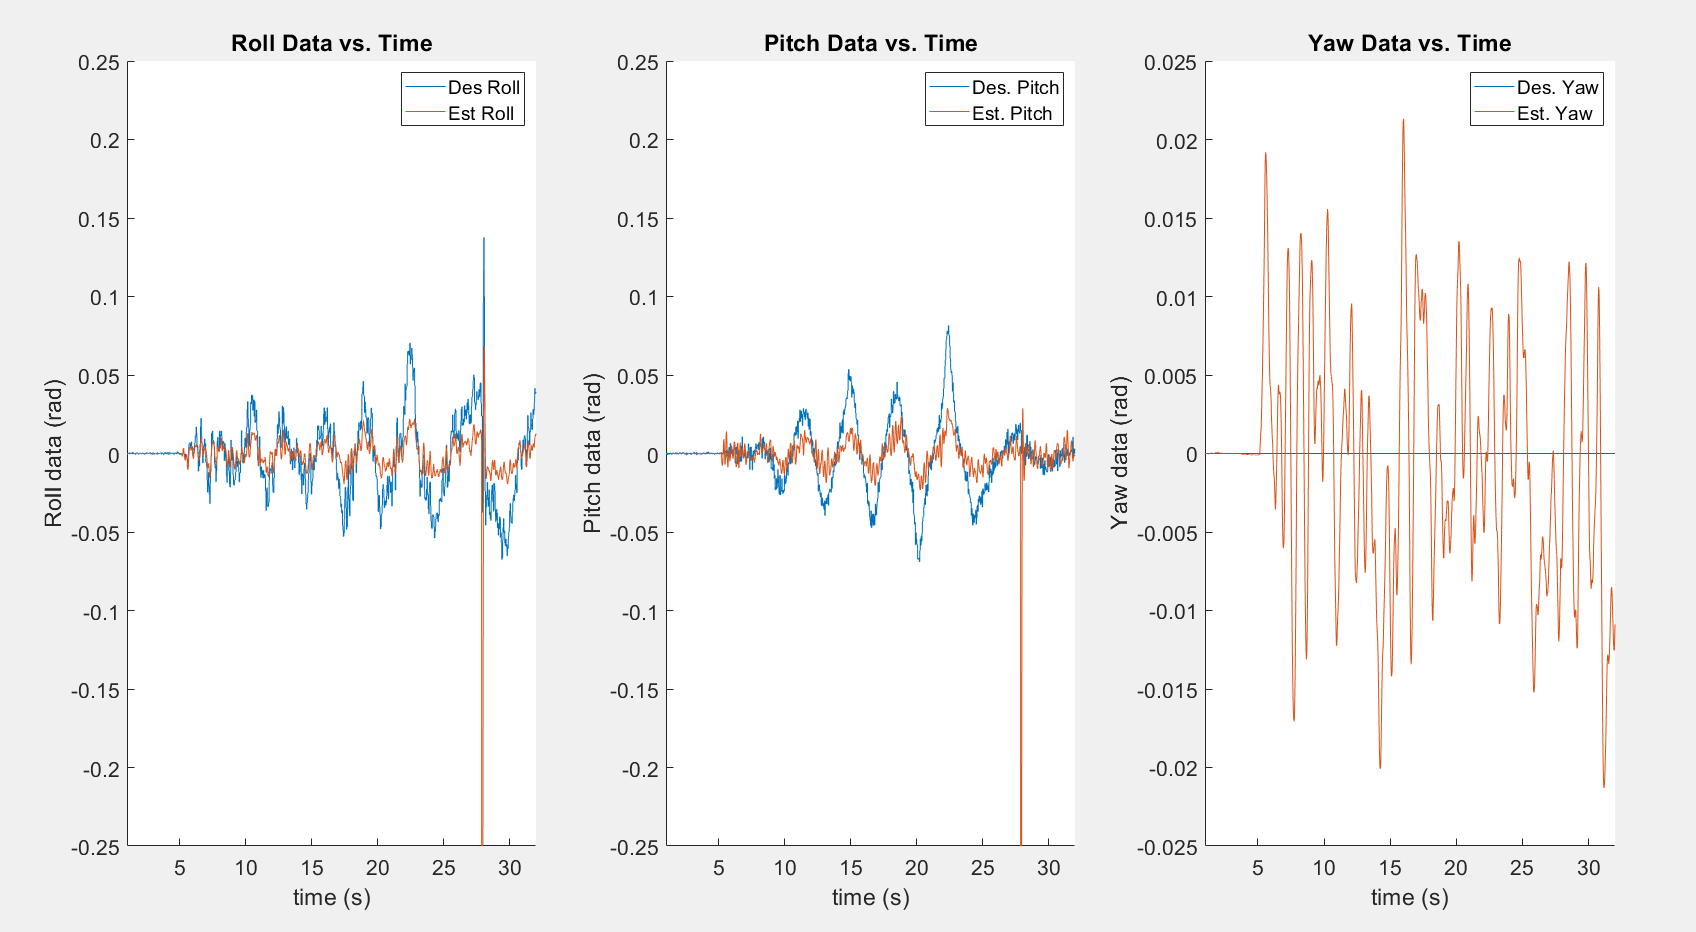
\includegraphics[scale=.34]{ME136_Lab5_Q5bi.png}
\caption{Estimated and Desired Angles VS Time}
\end{figure}
\FloatBarrier
\vspace{24pt}

\item The estimated vehicle velocity
\begin{figure} [H]
\centering
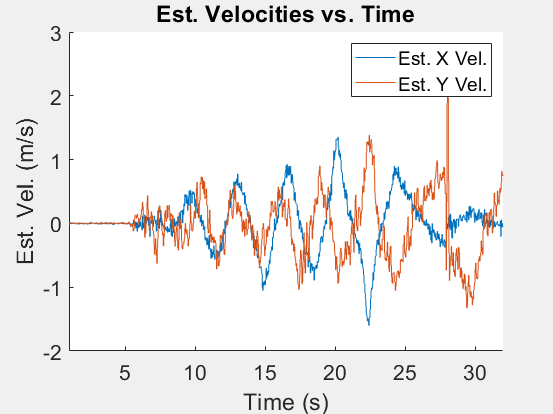
\includegraphics[scale=.75]{ME136_Lab5_Q5bii.png}
\caption{Estimated Vehicle Velocities VS Time}
\end{figure}
\FloatBarrier
\vspace{24pt}

\item The estimated height and desired height
\begin{figure} [H]
\centering
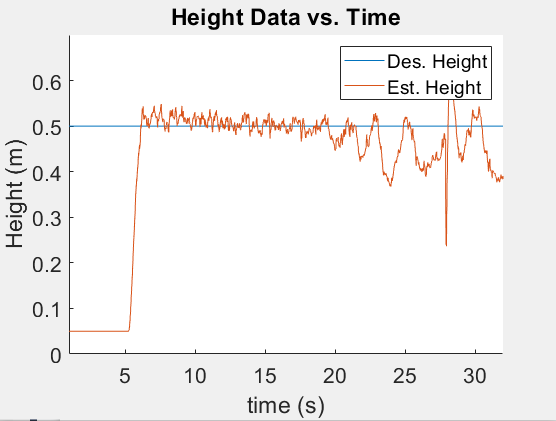
\includegraphics[scale=.75]{ME136_Lab5_Q5biii.png}
\caption{Height Data VS Time}
\end{figure}
\FloatBarrier
\vspace{24pt}

\item The total motor force
\begin{figure} [H]
\centering
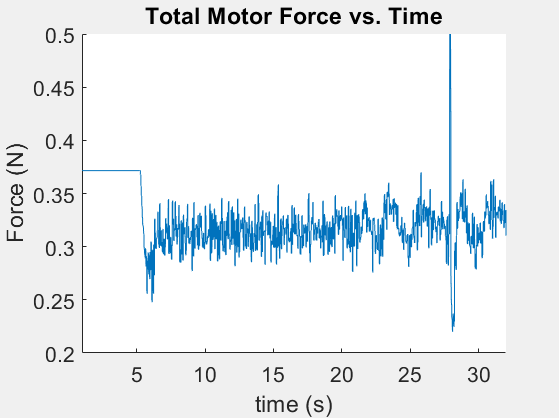
\includegraphics[scale=.75]{ME136_Lab5_Q5biiii.png}
\caption{Motor Command Values VS Time}
\end{figure}
\FloatBarrier
\vspace{24pt}

\end{itemize}


\subsection{Part C}

After some modification to the constants in our code, our results remained stable for an average 30 seconds. Initially, with the initial code in Lab 5, the glider would avoid hitting the wall for up to 5 seconds. While in the 30 seconds, the glider can start to swing aggressively before hitting the wall, its ability to correct clearly outperforms the initial test. 

\subsection{Part D}

Our code deviated from the standard in two main ways: We made slight changes to the time constants and large change to the mixer height and horizontal velocity. Our final values for time constants were as follows: Roll rate  = 0.035, Yaw rate = 0.15, Roll angle = 0.097, Yaw angle = 0.2. The mixer values saw more comprehensible change with our mixer height value at 0.3 and the mixer horizontal velocity value at 0.7. A "binary search" style iteration allowed our group to test small changes in the time constants to arrive at values that resulted in the best stability. Any change that kept the drone from hitting the walls was kept and continued until the improvements diminished. This iterative method produced our optimal numbers which kept the drone afloat for around 12 seconds on average. The mixer values however created a far more substantial improvement. The horizontal velocity value in particular resulted in dulled reaction in response to estimated velocity and prevented the drone from overcompensating from the control errors it was seeing. These two changes combined resulted in significant stable flight times. 

\section{Analysis and Modifications}
\subsection{Part A}
As stated in section 5.4, our code diverged from the standard in two key ways: We made slight adjustments to the time constants and implemented significant changes to the mixer height and horizontal velocity. The finalized values for the time constants were as follows: Roll rate = 0.035, Yaw rate = 0.15, Roll angle = 0.097, Yaw angle = 0.2. The mixer values underwent more discernible modifications, with the mixer height set at 0.3 and the mixer horizontal velocity at 0.7. Employing a "binary search" style iteration enabled our group to systematically test minor alterations in the time constants, ultimately yielding values that optimized stability. Any modification preventing the drone from colliding with walls was retained, and the process continued until further enhancements became marginal. This iterative approach led to our optimal parameters, allowing the drone to remain airborne for an average of approximately 12 seconds. However, the mixer values brought about a significantly more pronounced improvement. Particularly, the adjustment in horizontal velocity resulted in a dampened response to estimated velocity, preventing the drone from overcompensating for observed control errors. The combination of these two alterations resulted in notably extended stable flight times.

\subsection{Part B}

From our testing, the main limitation is the size of the drone. Our vehicle was losing stability due to over-correction. Originally the drone would tend to spiral in a circular pattern till it hit the wall but as our stability improved the motion became more of a swing. We believe that if we could increase the length of the propeller arms, the drone would better correct the motion generated from the noise. Also, if given more space, we believe the drone would better stabilize. This swinging motion would often nearly correct itself if given the time, however it often would hit the wall when swinging widely to compensate, prevent the correction. While this is still certainly unstable, we believe the airtime would increase exponentially with the expansion of the room.

\subsection{Part C}

To evaluate the improvements on the drone's stability, we plotted all the output values for every test run in MATLAB and viewed the estimated data and measured data together when applicable. These values gave us concrete information on what changes were successful, and what hindered the stability. Two example plots from past test runs are below:


\begin{figure} [H]
\centering
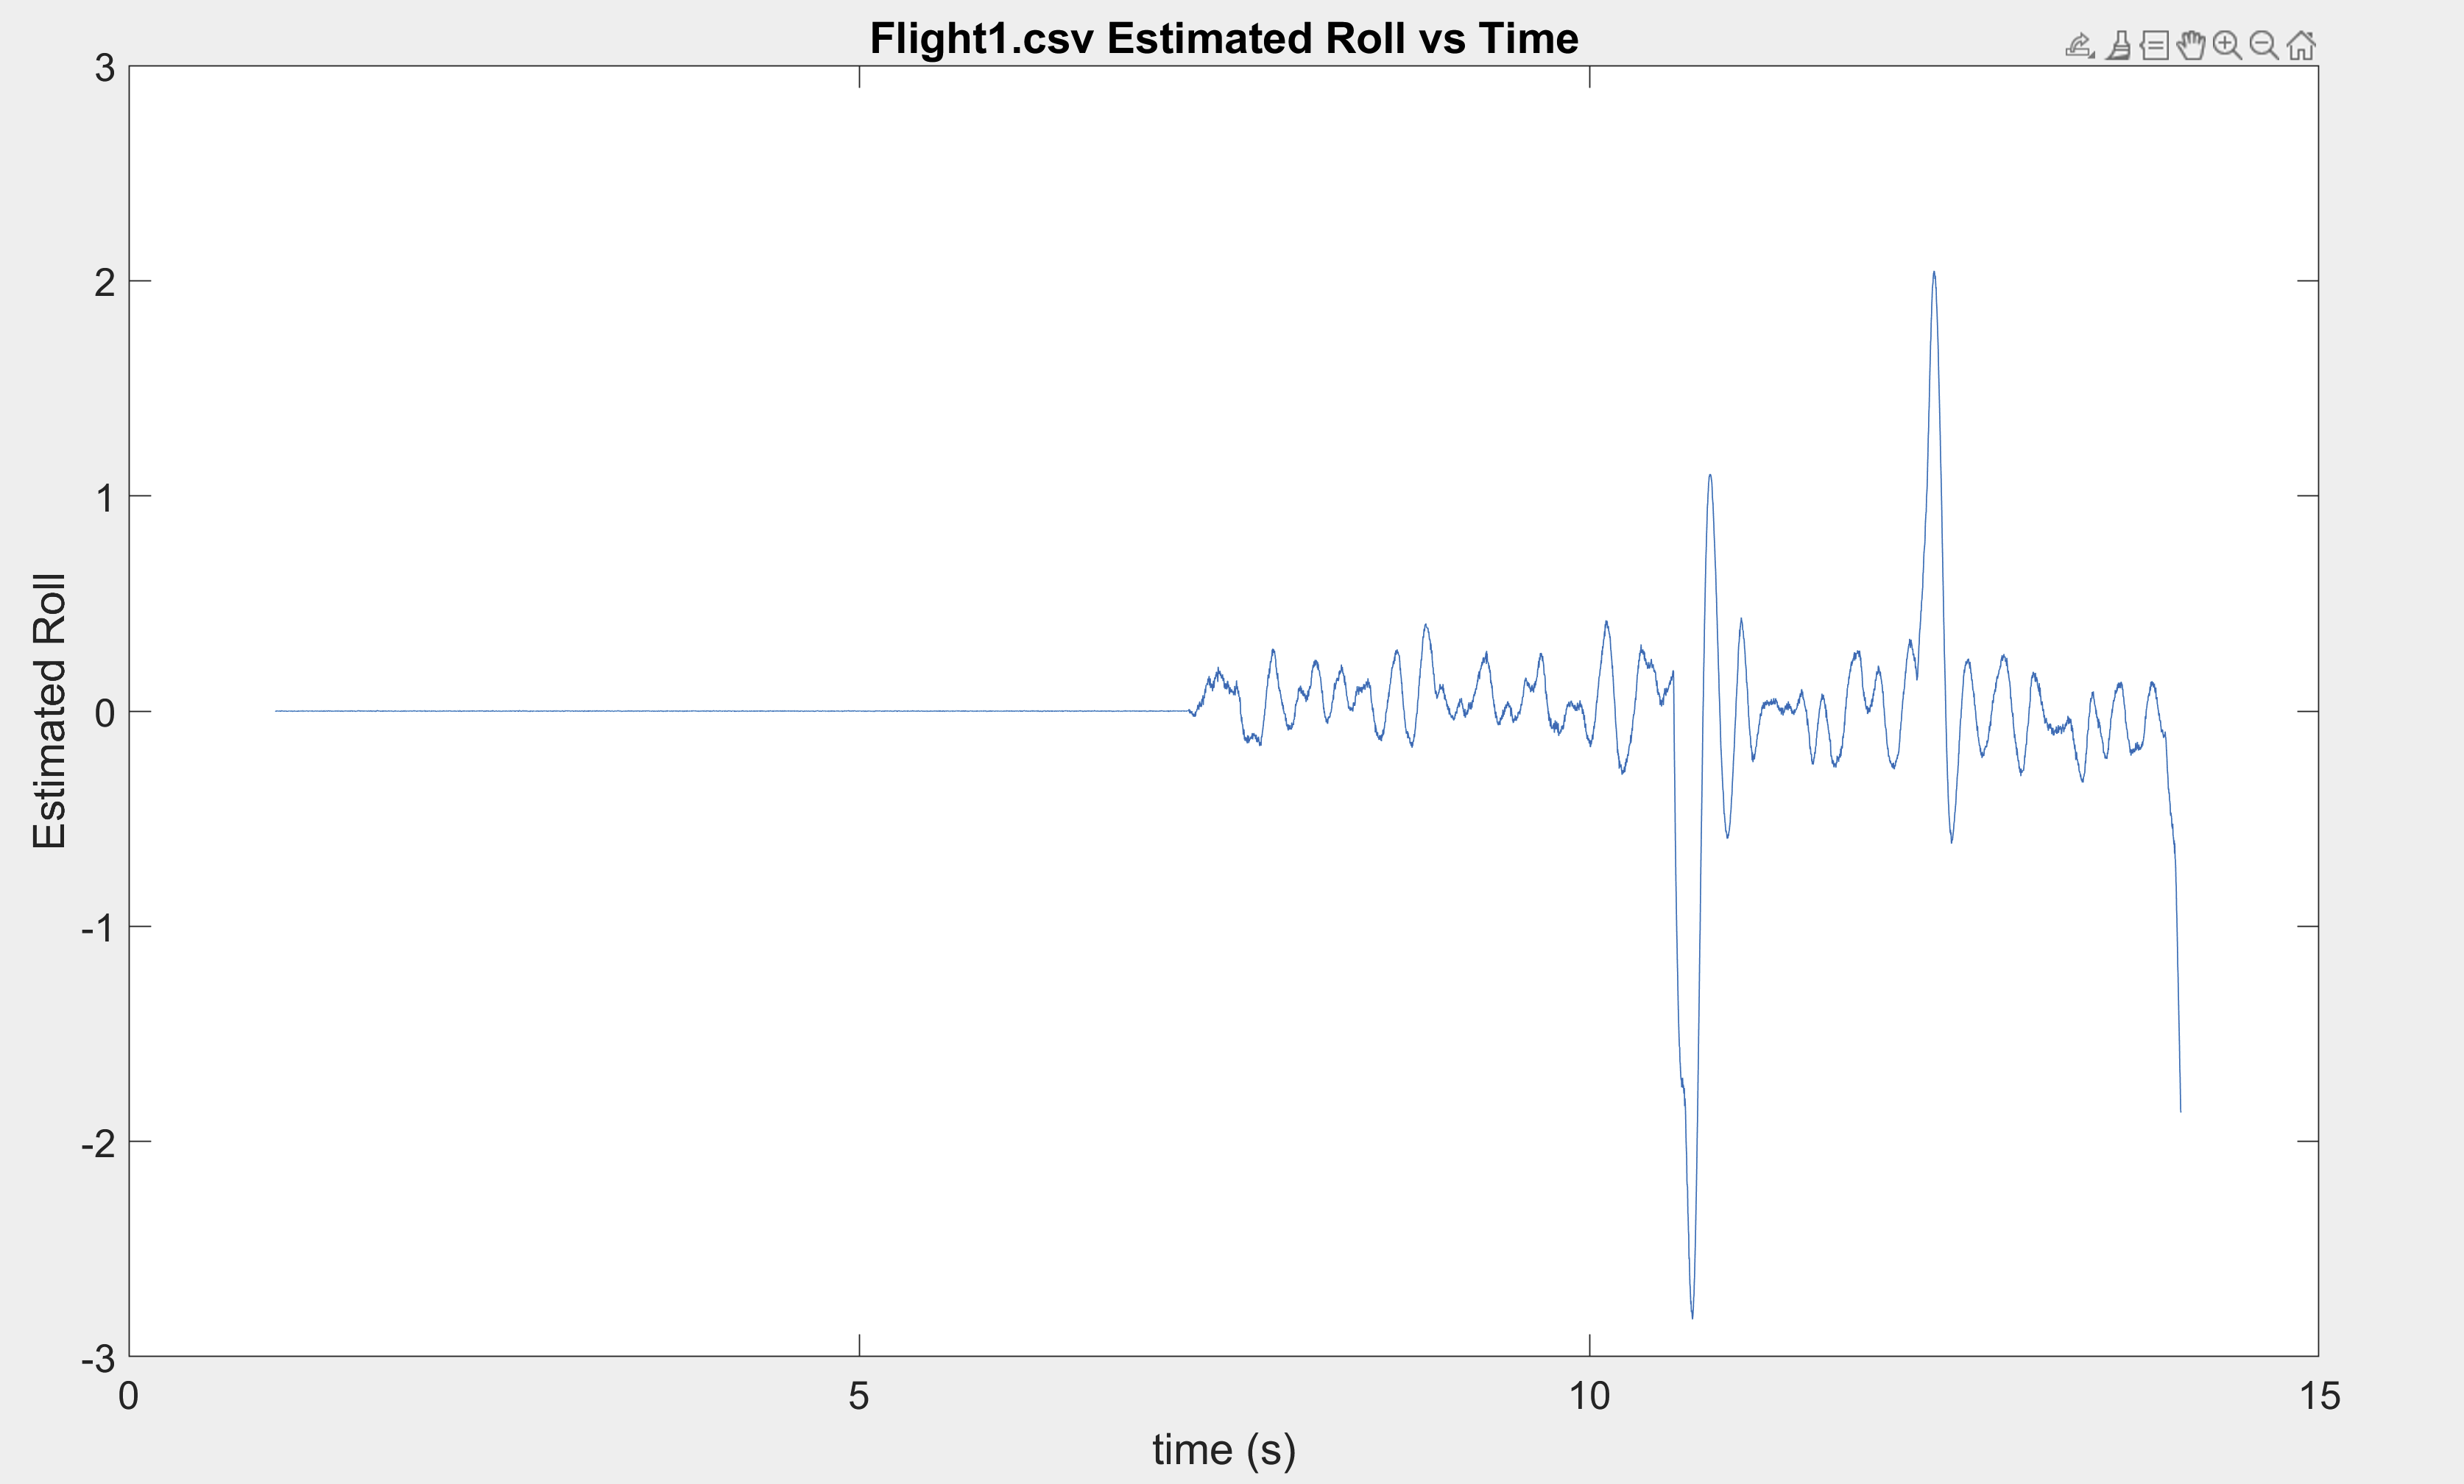
\includegraphics[scale=.12]{roll1.png}
\caption{Test 1 Roll vs Time}
\end{figure}
\FloatBarrier
\vspace{24pt}


\begin{figure} [H]
\centering
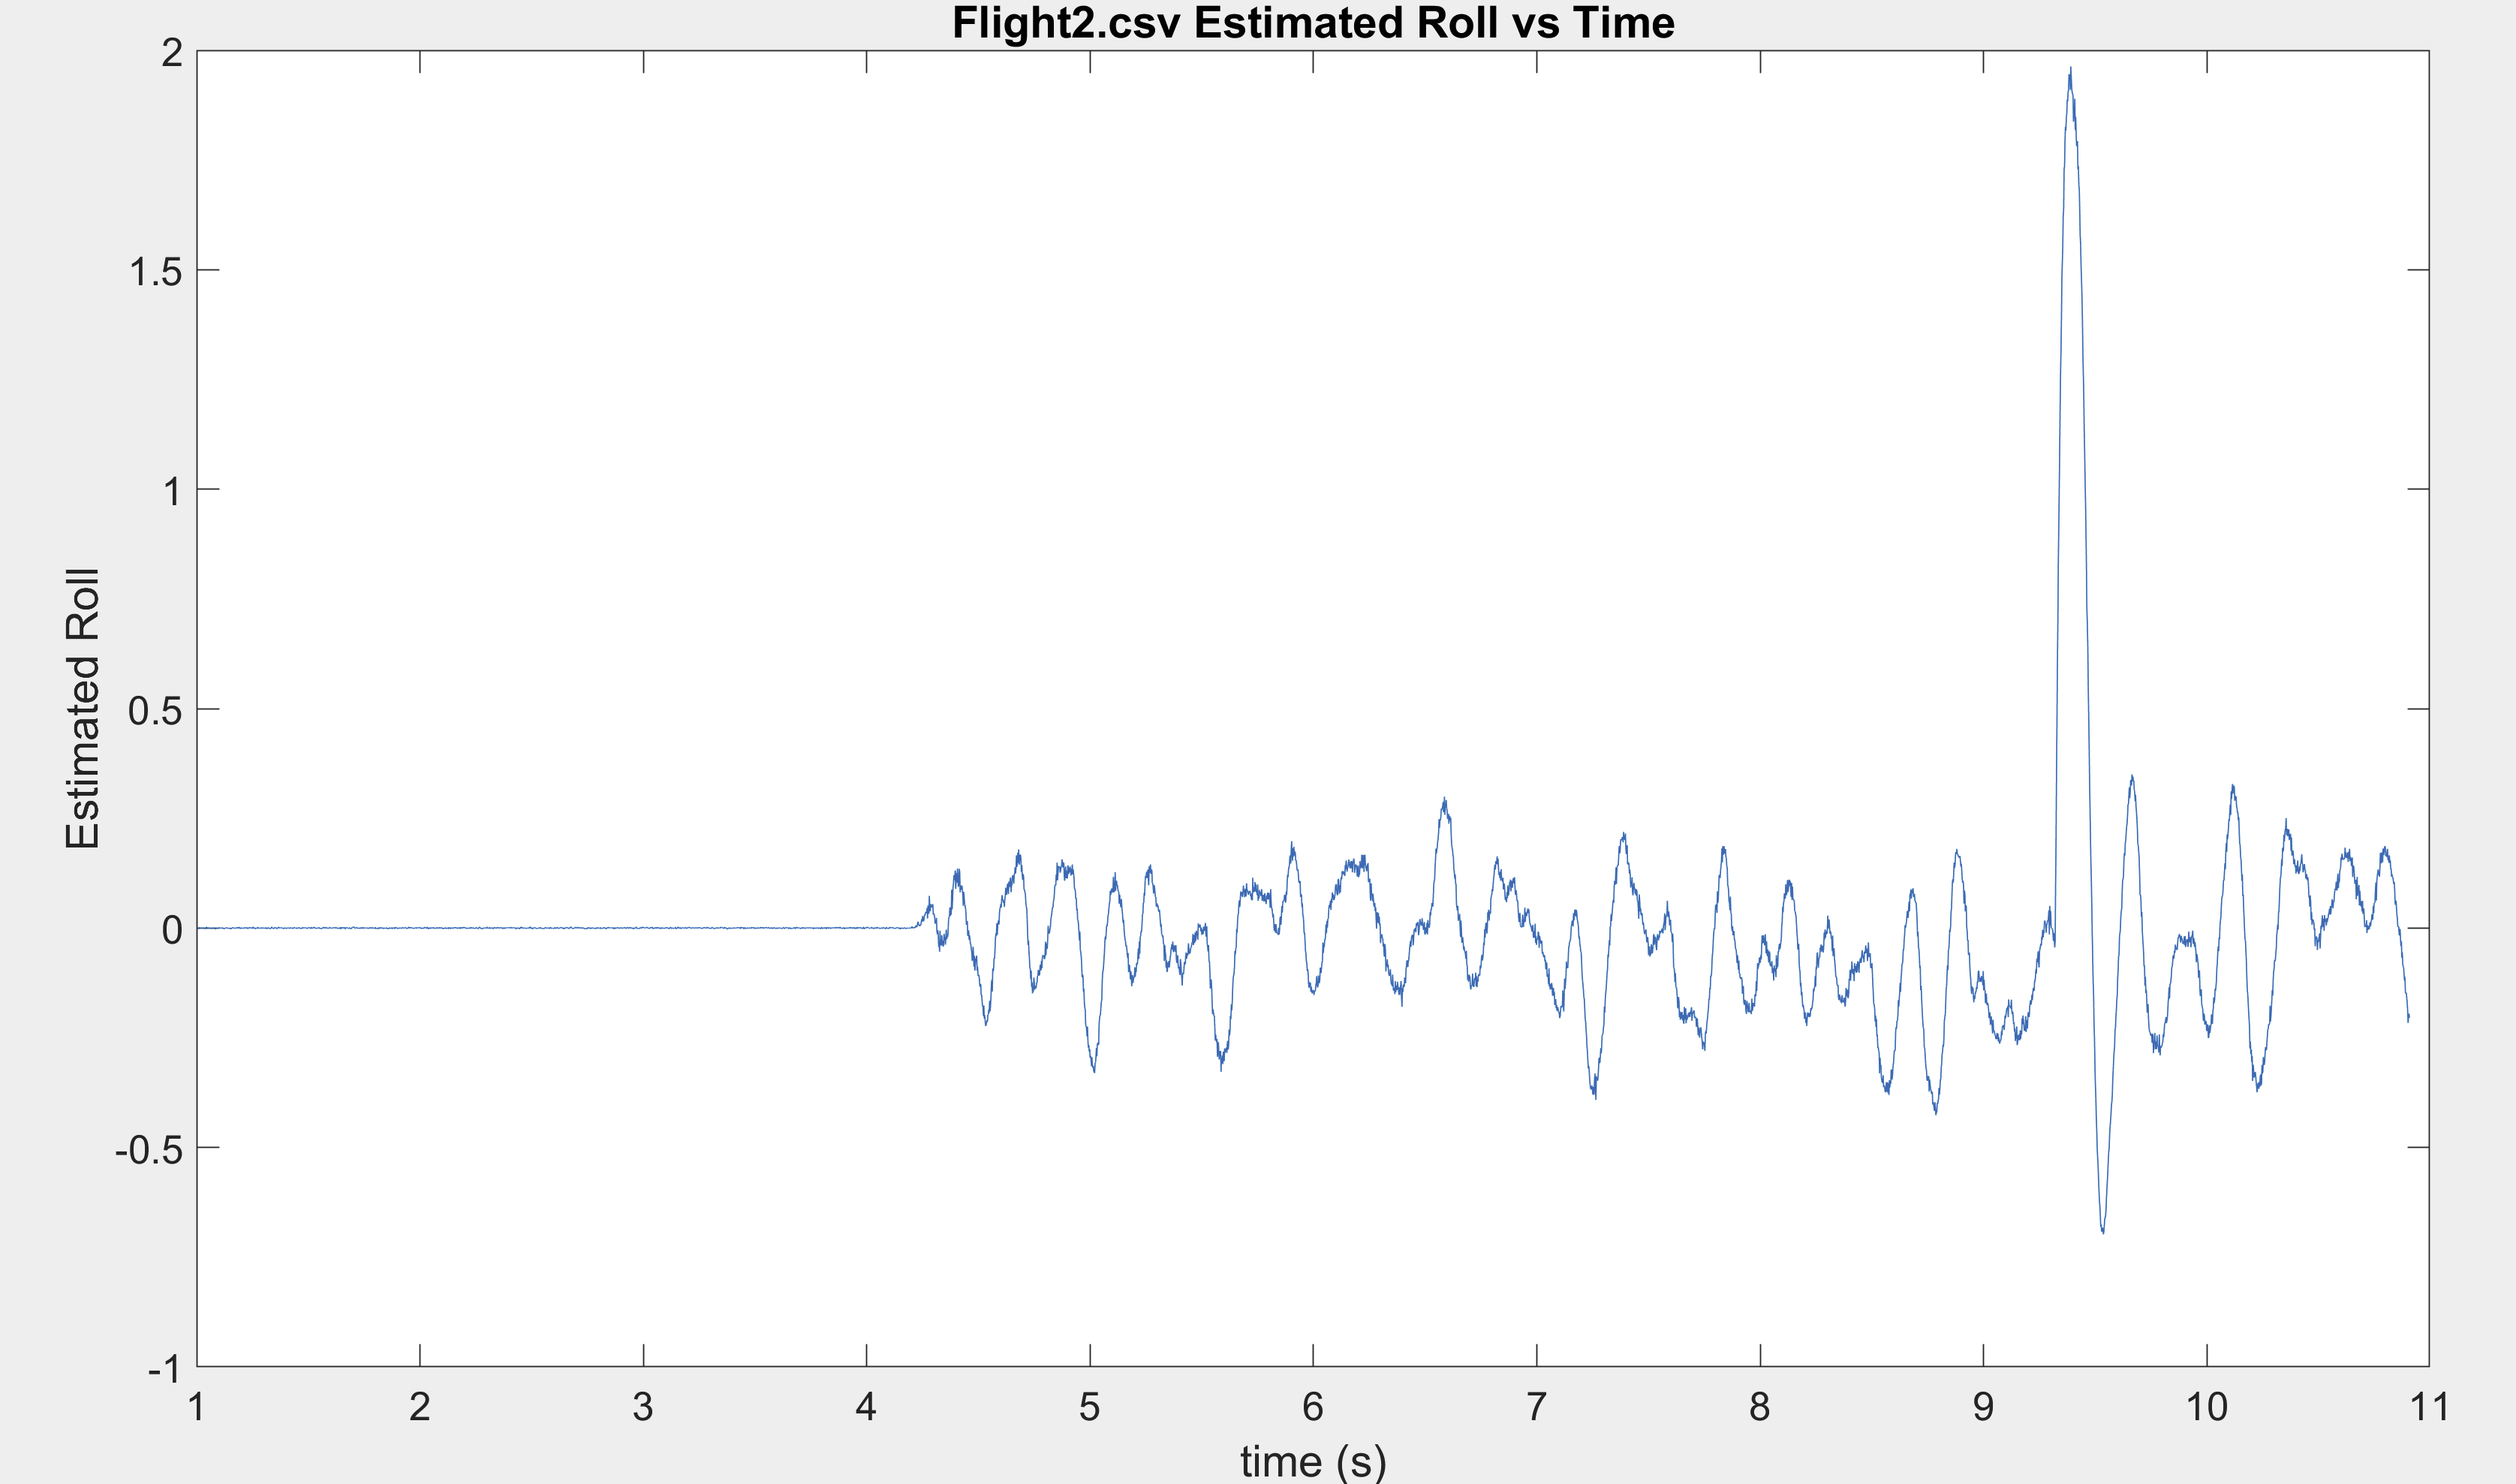
\includegraphics[scale=.12]{roll2.png}
\caption{Test 2 Roll vs Time}
\end{figure}
\FloatBarrier
\vspace{24pt}



\section{MainLoop Function}

\subsection{Virtual Machine Code}

On the page below is the full listing of our UserCode with comments where we added code for lab 5 starting on the second page:
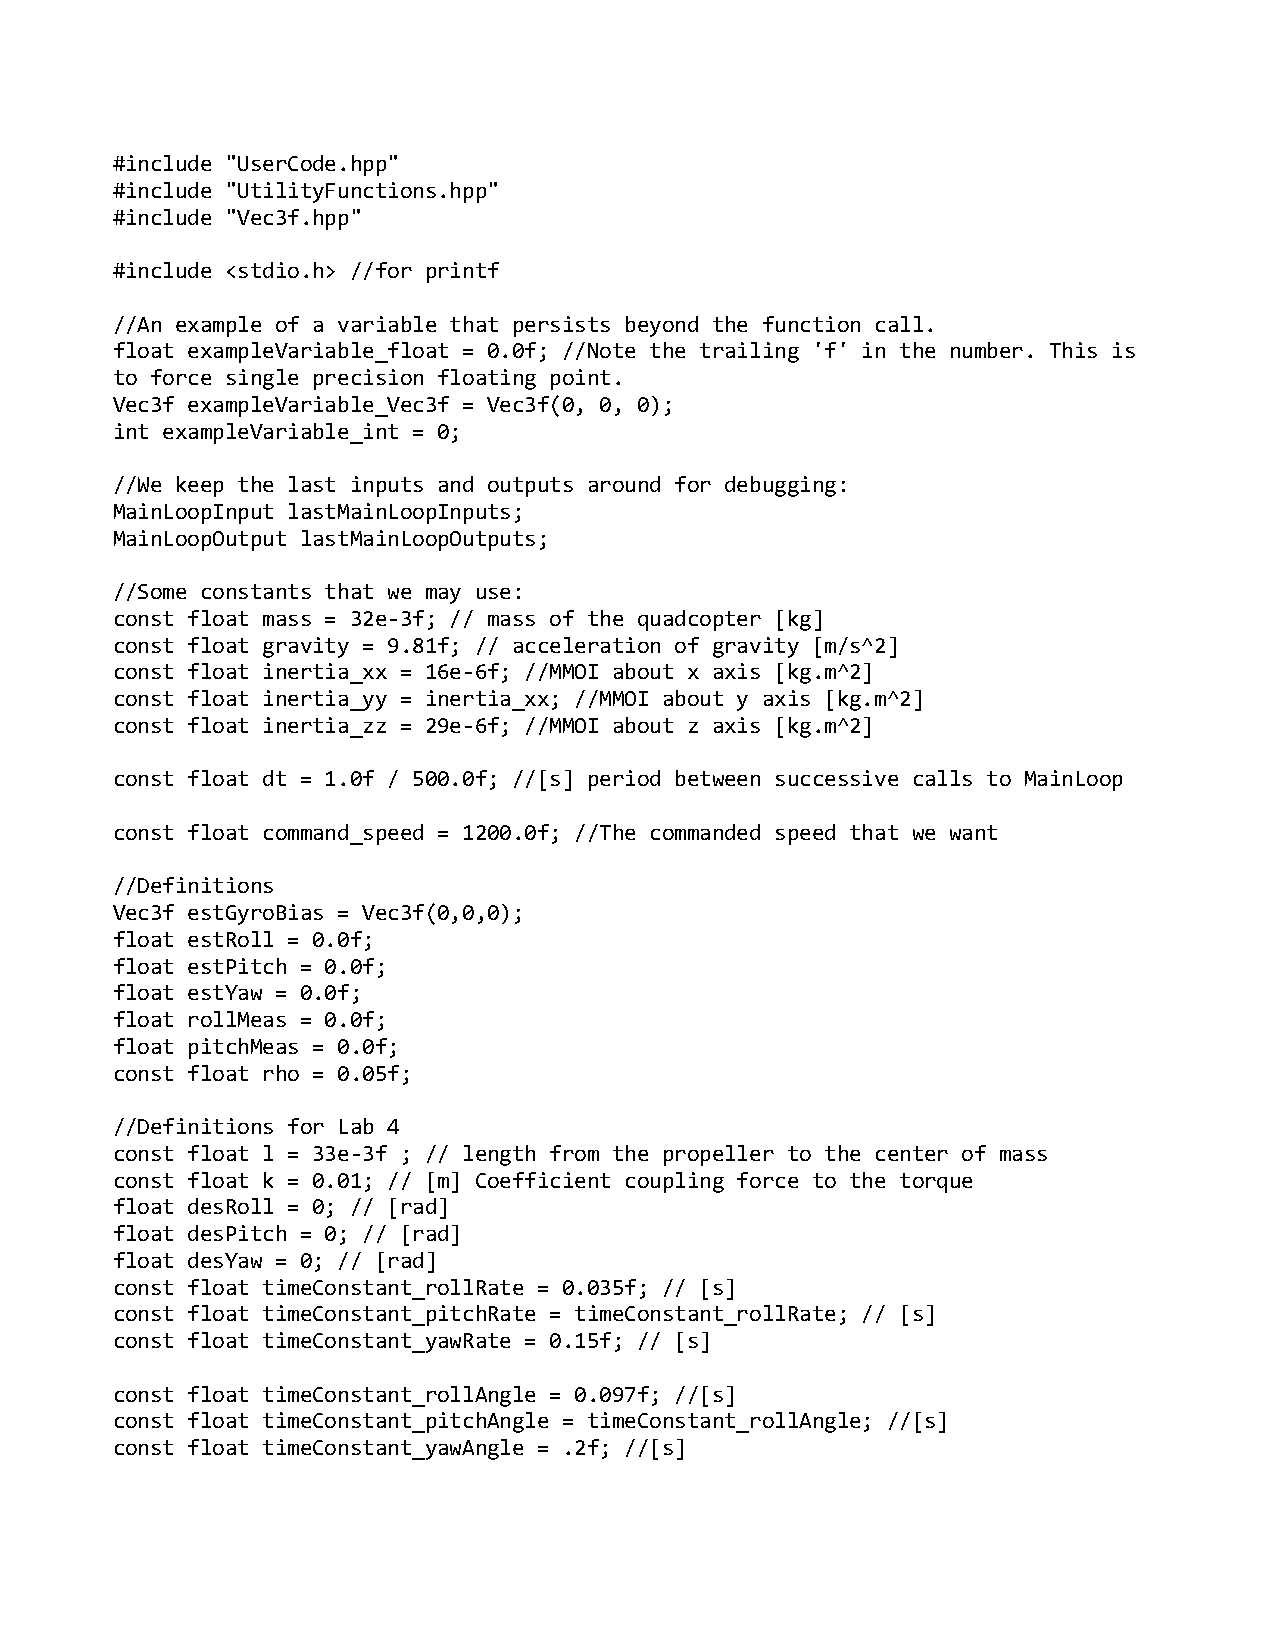
\includepdf[pages=-]{ME136_Lab5_UserCode.pdf}

On the page below is the full listing of our UtilityCode with comments:
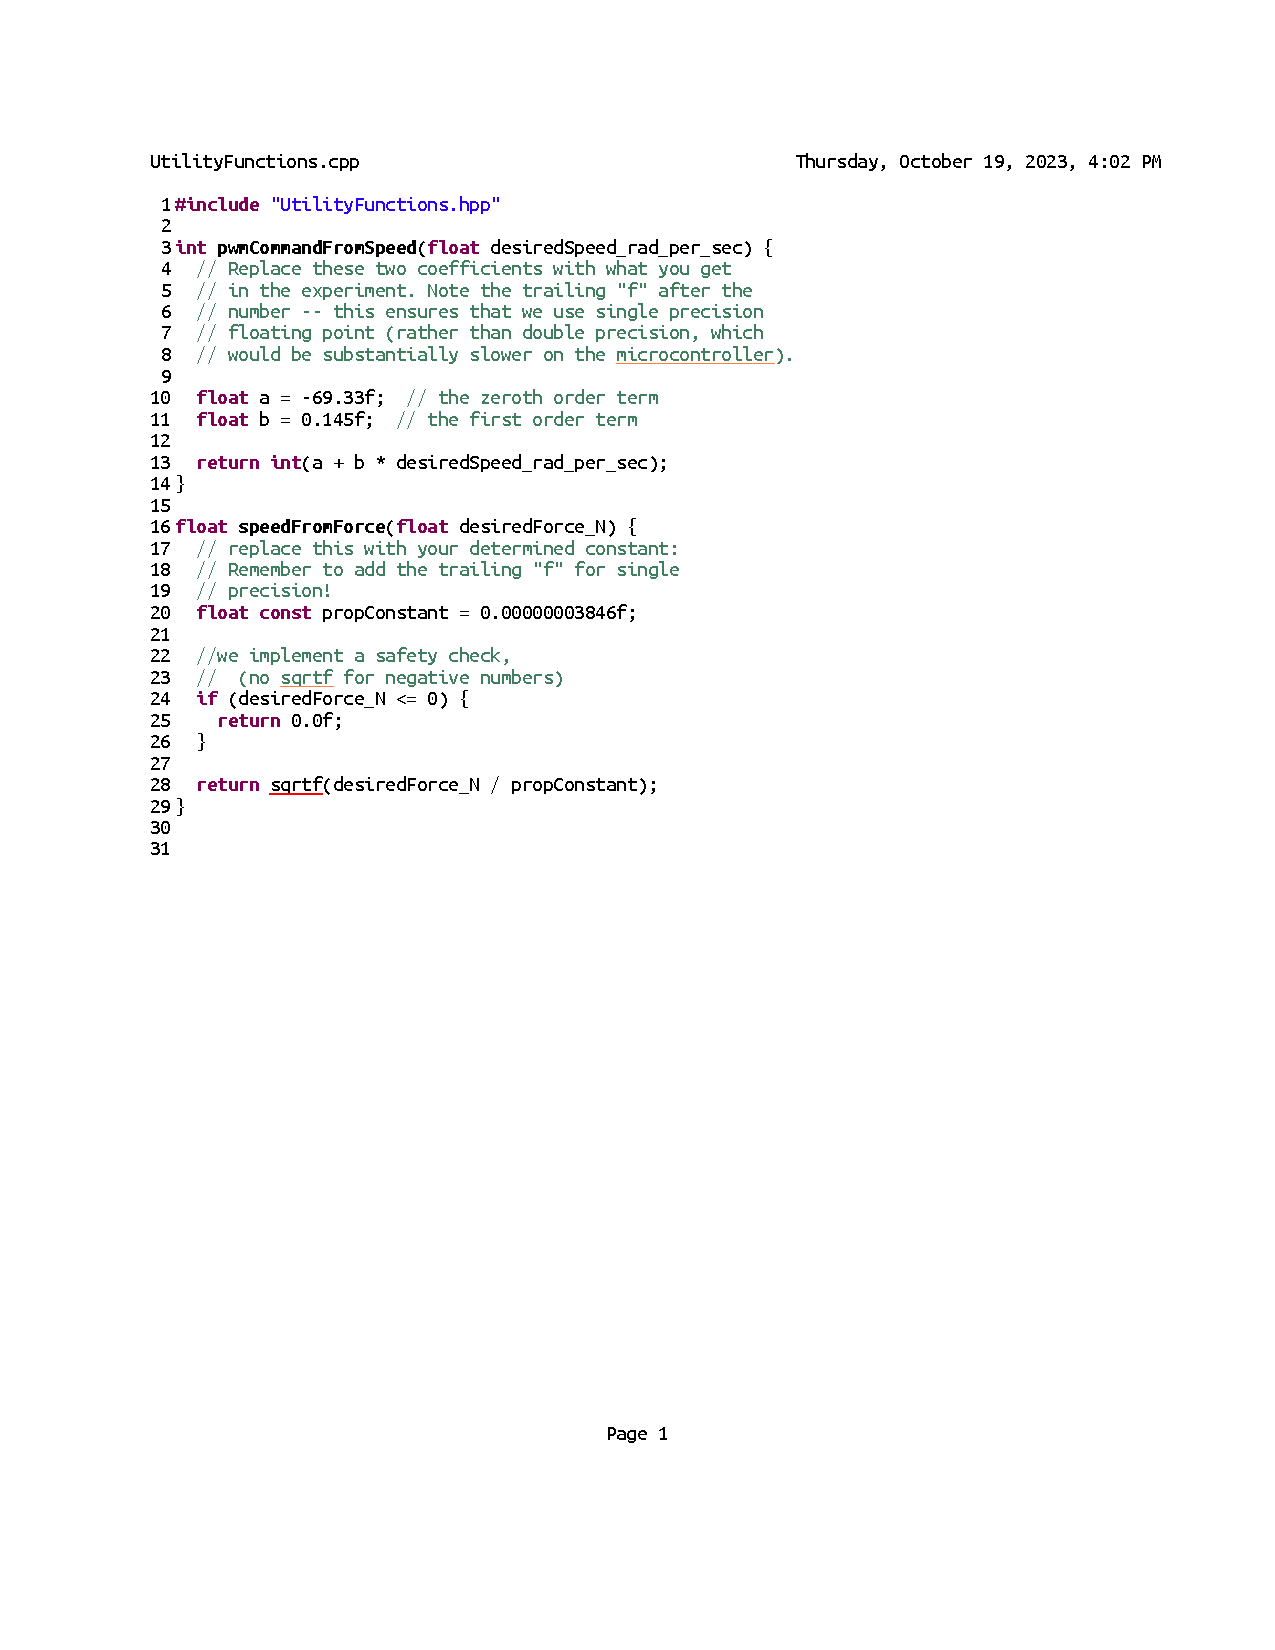
\includepdf[pages=-]{Lab4UtilityCode.pdf}

\subsection{Matlab Code} 
On the page below is our Matlab code we used to plot our deliverables.

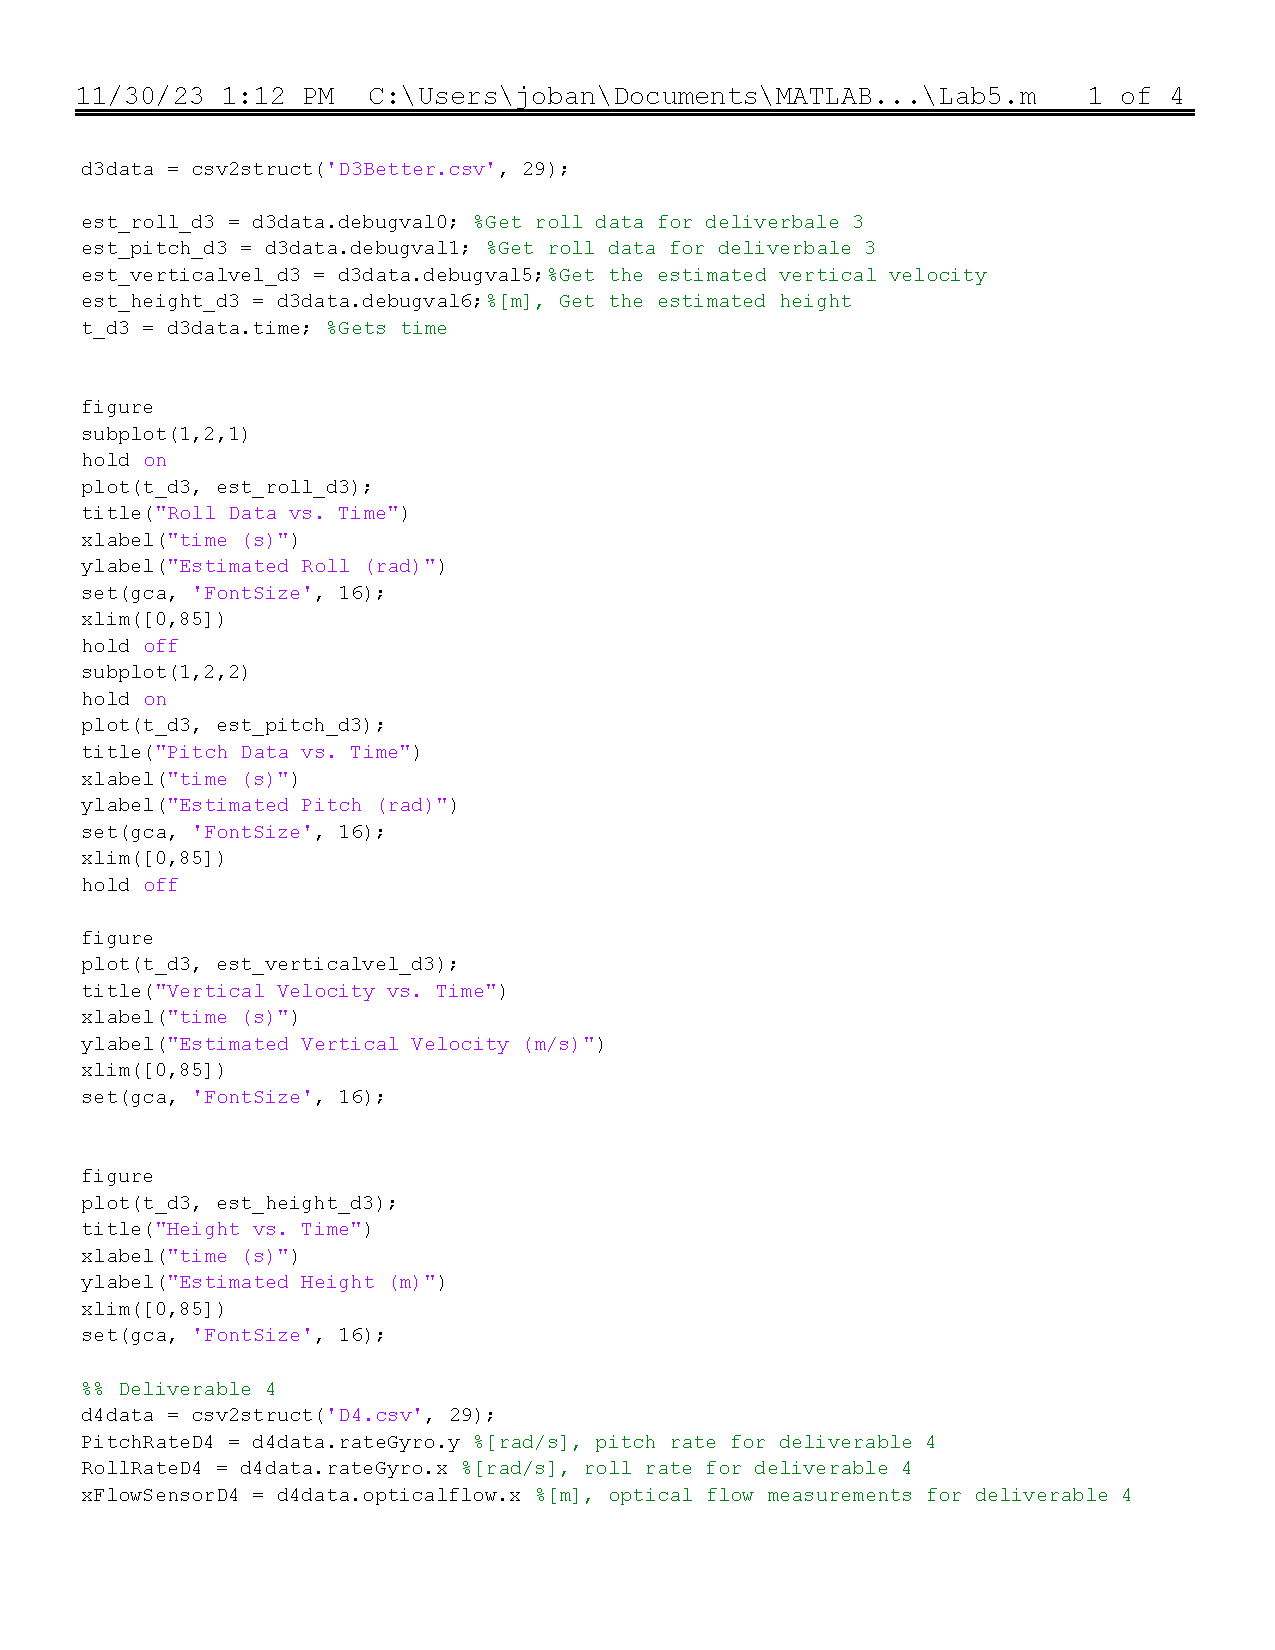
\includepdf[pages=-]{Lab5MatlabCode.pdf} 

\end{document}

